\documentclass[12pt,fleqn]{article}\usepackage{../common}
\begin{document}
Ders 14

Bagimsiz Olmayan Degiskenler (Non-independent Variables)

Ornek

Fizikteki $f(P,V,T)$ formulu, ki bu degiskenler 

\[ PV = nRT \]

seklinde ilintili. Daha genel olarak bir $f(x,y,z)$ formulu var, ve
degiskenler $x,y,z$ birbiriyle $g(x,y,z) = c$ uzerinden baglantili. Aslinda
bir onceki dersteki ayni durum, sadece bu sefer min, maks degil, kismi
turevlere neler oldugunu inceleyecegiz. 

Yine onceki dersteki gibi, belki $g$'yi cebirsel olarak degistirip, $f$'e
sokup degisken yoketmek mumkun degil. Eger oyle yapabilsek, bir $z =
z(x,y)$ 
olabilirdi, ve onun kismi turevlerine bakabilirdik,

\[ \frac{\partial z}{\partial x}, \frac{\partial z}{\partial y}, .. \]

gibi. Peki ya $z$'yi bulamiyorsak? Belki ustteki kismi turevleri $z$'yi
bulmadan elde edebiliriz. 

Ornek

\[ x^2 + yz + z^3 = 8 \]

$(2,3,1)$ noktasina bakalim (yerine koyunca hakikaten 8 ciktigini
goruyoruz). Fakat bu degerlerde azicik degisiklik yapinca, $z$ nasil
degisir? Bu soruyu nasil cevaplarim? 

Formulden $z$'yi cekip cikarmak gerekir, kupsel (cubic) formullerde bunu
yapmanin bir yolu var, fakat cok karmasik bir formul ortaya
cikartiyor. Aradigimiz sonuca ulasmanin daha kolay bir yolu var. 

$g$'nin tam diferansiyeline, yani $dg$'ye bakalim (ustteki formulu $g$
kabul ediyoruz). Tam diferansiyel

\[ 2x dx + z dy + (y+3z^2) dz = 0\]

Sag taraf sifir cunku ustteki $g$ bir sabite esit, $g=8$, sabitin degisimi
sifir, yani $dg=0$. 

Tam diferansiyele $(2,3,1)$ degerini verelim

\[ 4dx + dy + 6dz = 0 \]

Bu formul bize her degiskenin degisiminin digeri ile nasil baglantili
oldugunu gosteriyor. Mesela $dx$ ve $dy$'yi biliyorsak, $dz$'yi, yani
$z$'nin degisimini hesaplayabiliriz. Yani $z=z(x,y)$ uzerinden 

\[ dz = -\frac{1}{6}(4dx + dy) \]

Bu formul bize kismi turevleri de gostermis oluyor aslinda, cunku tam
diferansiyel formulunde kismi turevler vardir, ustteki formulde $dx,dy$'nin
yaninda yer alan degerler onlardir. O zaman

\[ \frac{\partial z}{\partial x} = -\frac{4}{6} = -\frac{2}{3} \]

\[ \frac{\partial z}{\partial y} = -\frac{1}{6} \]

Bunu dusunmenin bir diger yolu su. $\partial z/\partial x$ $z$'nin $x$'e
gore degisimi ise, $y$ sabit demektir, ustteki $dz$ formulunde $dy=0$
deriz, geri kalanlar

\[ dz = -\frac{2}{3}dx \]

ki bu formul $z$'nin $x$'teki degisime gore nasil degistigini gosteriyor. 

Genel olarak 

\[ g(x,y,z) = c \]

ise, o zaman 

\[ dg = g_x dx + g_y dy + g_z dz \]

formulu sifira esitlenir, ve bir diferansiyel digerinin formunda elde
edilebilir. 

\[ dz = -\frac{g_x}{g_z}dx -\frac{g_y}{g_z}dy \]

O zaman $\frac{\partial z}{\partial x}$'i gormek istiyorsak, $dx$'in katsayisina bakabiliriz, ya 
da $y=sabit$ yani $dy=0$ deriz, ve geri kalanlar

\[ dz =  -\frac{g_x}{g_z}dx, \ 
\frac{\partial z}{\partial x} = -\frac{g_x}{g_z}dx
\]

Daha fazla ilerlemeden, simdiye kadar gordugumuz notasyonun bazi
problemlerini inceleyelim. 

\[ f(x,y) = x+y \]

\[ \frac{\partial f}{\partial x} = 1\]

Degisken degisim (change of variables) yapalim

\[ x = u \]

\[ y = u+v \]

Pek cetrefilli bir degisim degil bu. O zaman 

\[ f = x + y = 2u + v \]

\[ \frac{\partial f}{\partial u} = 2\]

Bu nasil oldu? $x=u$ dedigimize gore, $x,u$ birbiriyle esitler, o zaman
kismi turevleri de ayni olmaliydi. 

Bu uyusmazligin niye ortaya ciktigini anlamak icin notasyonun ne demek
istedigine yakindan bakmamiz lazim. $\partial f/\partial x$ ile $x$'i degistiriyor, 
ama $y$'yi sabit tutuyoruz. $\partial f/\partial u$ ile $u$'yu degistiriyor, ama $v$'yi 
sabit tutuyoruz.

Yani evet, $x$ ile $u$'yu degistirmek ayni sey olabilir, ama $v$'yi sabit
tutmak ile $y$'yi sabit tutmak ayni sey degildir. Cunku mesela $y$'yi sabit
tutarsam ve $u$'yu degistirirsem, $v$ de degismelidir (ki biz bunu
istemiyoruz) $y = u+v$ ifadesindeki toplaminin sabit kalmasi icin. Ya da $v$ 
sabit ise ve $u$'yu degistiriyorsam, $y$ degisecektir. 

Yani hos, guzel kismi turev notasyonumuz neyin degistigini acikca
gostermesine ragmen, neyin sabit tutuldugunu gostermedigi icin yanilgilara
yol acabiliyor. Bunu aklimizda tutmamiz lazim. Ornekteki kismi turevler
birbiriyle ayni degil cunku 

$\partial f/\partial x$, $u=x$'i degistir, ve $y$'yi sabit tut

$\partial f/\partial u$, $u=x$'i degistir, ve $v = y-x$'i sabit tut

anlamina geliyor. 

Daha acik bir notasyon soyle olabilir

\[ 
\bigg( \frac{\partial f}{\partial x}  \bigg)_y = \textrm { y sabit}
 \]

\[ 
\bigg( \frac{\partial f}{\partial u}  \bigg)_v = \textrm { v sabit}
 \]

Ornege donersek

\[ 
\underbrace{
\bigg( \frac{\partial f}{\partial x}  \bigg)_y 
}_{1} 
\ne 
\underbrace{
\bigg( \frac{\partial f}{\partial x}  \bigg)_v = 
\bigg( \frac{\partial f}{\partial u}  \bigg)_v 
}_{2}
 \]

Ornek

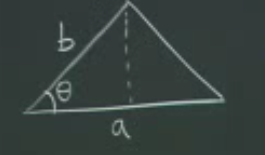
\includegraphics[height=2cm]{14_1.png}

\[ A = \frac{1}{2}absin(\theta) \]

Alan, $a,b,\theta$'nin fonksiyonu. 

Farz edin ki size $a,b,\theta$ arasinda bir iliski oldugunu soyledim. 

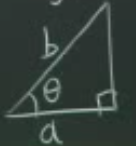
\includegraphics[height=2cm]{14_2.png}

Diyelim ki ucgen aslinda bir dik ucgen, bunu cebirsel olarak soylemenin
yolu da alttaki kisitlama ifadesi

\[ a = bcos(\theta) \]

Incelemek istedigimiz alanin $\theta$'ya olan baglantisi, yani, mesela
$A$'nin degisiminin $\theta$'nin degisimine orani nedir? Bunu hesaplamanin
3 yontemi olabilir

1) $a,b,\theta$'yi bagimsiz kabul et, o zaman

\[ \frac{\partial A}{\partial \theta} = 
\bigg( \frac{\partial A}{\partial \theta} \bigg)_{a,b}  \]

Tabii $a,b$ sabitken $\theta$ degissin demek, ucgenin dikliginin ihlali
demektir, cunku hem kenarlar sabit, hem aci degissin diyoruz, ama o zaman
dik aci degismek zorundadir. Her neyse, kismi turevleri hesaplayalim. 

\[ \frac{\partial A}{\partial \theta} = \frac{1}{2}ab cos(\theta) \]

Simdiye kadar kisitlama ifadelerimi kullanmadim. 

2) $a$'yi sabit tutalim, $b$ degisebilsin, ki boylece dik aci yerinde
kalabilsin. 

\[ b = b(a,\theta) = \frac{a}{cos(\theta)} \]

\[ \bigg( \frac{\partial A}{\partial \theta} \bigg)_{a}  \]

3) $b$'yi sabit tutalim, $a = a(b,\theta)$ degissin, ki boylece dik aci yerinde
kalabilsin. 

\[ \bigg( \frac{\partial A}{\partial \theta} \bigg)_{b}  \]

Bunlardan bir tanesini hesaplayalim, mesela $\bigg( \frac{\partial A}{\partial \theta} \bigg)_{a} $.

Hesabi yapmanin uc degisik yolunu gorecegiz. 

0. Metot: $b$'yi yanliz birak (cebirsel), ve diger formule sok

\[ a = b \ cos (\theta) => b = \frac{a}{cos(\theta)} = a \ sec (\theta)\]

\[ A = \frac{1}{2} \ ab \ sin(\theta) \]

\[ = \frac{1}{2} \frac{a^2 sin(\theta)}{cos(\theta)} \]

\[ = \frac{1}{2} a^2 tan(\theta) \]

O zaman 

\[ \bigg( \frac{\partial A}{\partial \theta} \bigg)_{a} = 
\frac{1}{2}a^2sec^2(\theta)
 \]

Bu arada $sec$, $1/cos$ demektir, eger ve onun turevini $1+tan^2$ olarak
biliyorsaniz, o da ayni kapiya cikar. 

Hoca bu metotu tavsiye etmiyor (onun icin metot sayisi biraz espri yaparak
'sifir' vermis) cunku her zaman yanliz birakma, baska formule sokma mumkun
olmayabilir.

1. Metot: Diferansiyelleri Kullan

Yapilacaklar sunlar

- $a$'yi sabit tut, $da = 0$

- kisitlama ifadesi $a = b \ cos(\theta)$

Ustteki ifadenin diferansiyelini alalim

\[ da = cos(\theta) db - b \ sin(\theta) d\theta \]

Simdi elimizde $da,db,d\theta$'yi iliskilendiren bir ifade var. $a$'nin
sabit oldugunu biliyoruz, o zaman $da=0$

\[ 0 = cos(\theta) db - b \ sin(\theta) d\theta \]

$db$'yi yanliz birakabiliriz

\[ cos(\theta) db = b \ sin(\theta) d\theta \]

\[ db = b \ sin(\theta) d\theta \ / \ cos(\theta) \]

\[ db = b \ tan(\theta) d\theta  \]

Boylece $b$'nin $\theta$'ya gore degisim oranini bulduk. Bu ne ise yarar?
Ana formulu hatirlayalim, ve onun da diferansiyelini alalim

\[ A = \frac{1}{2} \ ab \ sin(\theta) \]

\[ dA = \frac{1}{2} \ b \ sin(\theta) da + 
\frac{1}{2} \ a \ sin(\theta) db + 
\frac{1}{2} \ ab \ cos(\theta)d\theta
 \]

$da = 0$ ise, ilk terim yokolur. 

\[ dA = 
\frac{1}{2} \ a \ sin(\theta) db + 
\frac{1}{2} \ ab \ cos(\theta)d\theta
 \]

Geri kalanlarda, $db$ var, ama biz $\theta$'ya gore degisimi istiyoruz,
$db$'yi orada gormek istemiyoruz. O zaman elimizdeki $db$ formulunu buraya
sokalim. 

\[ dA =  
\frac{1}{2} \ a \ sin(\theta) \ ( \ b \ tan(\theta) d\theta \ ) \ + 
\frac{1}{2} \ ab \ cos(\theta)d\theta
\]

\[ dA =  
\frac{1}{2} \ ab \ (sin(\theta) tan(\theta) +  cos (\theta) )d\theta
\]

Trigonometriden 

\[ dA =  
\frac{1}{2} \ ab \ (
\underbrace{sin(\theta) tan(\theta) +  cos (\theta)}_{sec(\theta)}
)d\theta
\]

Sonucu bulduk 

\[ \bigg( \frac{\partial A}{\partial \theta} \bigg)_{a} = 
\frac{1}{2} \ ab \ sec(\theta)
 \]

Ozetlemek gerekirse, sunlari yaptik

- $A$'yi $da,db,d\theta$ ile ifade et

- $a=sabit, \ da=0$ demektir.

- Kisitlama ifadesinin diferansiyelini al, $db$'yi yanliz birak. 

- $dA$'ya sok

2. Metot: Zincirleme Kanununu Kullan

\[ \bigg( \frac{\partial A}{\partial \theta} \bigg)_{a} = 
A_\theta \bigg( \frac{\partial \theta}{\partial \theta} \bigg)_{a} + 
A_a \bigg( \frac{\partial a}{\partial \theta} \bigg)_{a} + 
A_b \bigg( \frac{\partial b}{\partial \theta} \bigg)_{a} 
 \]

\[  = 
A_\theta \cancelto{1}{\bigg( \frac{\partial \theta}{\partial \theta} \bigg)_{a}} + 
A_a \cancelto{0}{\bigg( \frac{\partial a}{\partial \theta} \bigg)_{a}} + 
A_b \bigg( \frac{\partial b}{\partial \theta} \bigg)_{a}
 \]

Sifir olan kismi turev oyle oldu cunku $a$ sabit dedik. Son terimdeki
kismi turev icin kisitlama ifadesini kullanacagiz.

Soru 2J-1 a)

\[ w = x^2+y^2+z^2, \ z = x^2+y^2 \]

icin 

\[ \bigg( \frac{\partial w}{\partial y}  \bigg)_z \]

hesabini yapin, ve direk yerine gecirme (direct subsitution) teknigini
kullanin. 

Cevap 

Ustteki notasyon tum sabit tutulan degiskenleri hangileriyse gostermek
zorunda, burada sadece $z$'nin sabit tutuldugu soyleniyor, degisen $y$. O
zaman bagimli degisken $x$ olmalidir. Bu degiskeni yokedelim,

\[ z = x^2+y^2 \]

\[ x^2 = z - y^2 \]

Yerine koyalim

\[  w = (z-y^2)+y^2+z^2 \]

\[ = z + z^2 \]

O zaman kismi turev

\[ \bigg( \frac{\partial w}{\partial y}  \bigg)_z  = 0\]

olacaktir. 

Soru 2J-2 (b) (i)

Ustteki $w$ icin, 

\[ \bigg( \frac{\partial w}{\partial z}  \bigg)_y \]

hesabini yap ve zincirleme kanunu kullan. 

Cevap 

\[  \bigg( \frac{\partial w}{\partial z}  \bigg)_y  =
2x \  \bigg( \frac{\partial w}{\partial z}  \bigg)_y  +  2z
 \]

Diger yandan 

\[ z = x^2 + y^2 \]

var, bunun uzerinde de ayni turevi alalim. Tekrar duzenleyip istedigimiz
degiskeni belli bir tarafa almaya gerek yok, cunku yerine gecirme teknigi
kullanmiyoruz. Iki tarafin kismi turevini alinca

\[ 1 = 2x  \bigg( \frac{\partial w}{\partial z}  \bigg)_y  \]

\[ \frac{ 1}{2x}  = \bigg( \frac{\partial w}{\partial z}  \bigg)_y  \]

Ana formulun kismi turevinde ustteki formulu yerine koyalim

\[  \bigg( \frac{\partial w}{\partial z}  \bigg)_y  =
2x \  \frac{1}{2x}  + 2z
 \]

\[   =
1 + 2z
 \]

Soru 2J-4 b)

\[ w = x^3y - z^2t, \ \ xy = zt\]

icin

\[ \bigg( \frac{\partial w}{\partial t}  \bigg)_{x,z}  \]

hesabini yap, tam diferansiyel teknigini kullan. 

Cevap

Cozum icin her iki denklemin tam diferansiyelini alacagiz. Bagimli,
bagimsiz bilgisi ise ``diferansiyel yerine gecirme'' uyguladigimizda ise
yarayacak, yani daha once duz degisken uzeinden yaptigimiz degisimi, simdi
diferansiyeller uzerinden yapacagiz. Tam diferansiyeli mekanik bir sekilde
once yazalim

\[ dw = w_x dx + w_y dy + w_z dz + w_t td \]

Gerekli kismi turevleri alalim

\[ = 3x^2y dx + x^3dy - 2zt dz + -z^2 dt\]

Aynisi ikinci denklem icin 

\[ y dx + x dy = t dz + z dt \]

Bizden istenene gore $t,x,z$'nin bagimsiz, geri kalan $y$'nin bagimli
oldugunu anliyoruz. O zaman ustteki formulde $dy$'yi yanliz birakirsak ve
ana tam diferansiyel icinde yerine koyarsak, istedigimiz sonuca
erisecegiz. 

\[ y dx  = t dz + z dt = x dy\]

Yerine koyalim, ve gruplayalim

\[ = 3x^2ydx + x^2(tdz + zdt - ydx) - 2ztdz - z^2dt \]

\[ = (3x^2y  - x^2y)dx + (x^2t-2zt)dz + (x^2z-z^2)dt  \]

\[ = (2x^2y) dx + (x^2t-2zt) dz + (x^2z-z^2)dt  \]

Aradigimiz kismi turev $t$'ye gore, o zaman ustteki tam diferansiyel
aciliminda $dt$'nin katsayisina bakacagiz. Orada $x^2x-z^2$ yaziyor, demek
ki aradigimiz sonuc bu. 

\[ \bigg( \frac{\partial w}{\partial t}  \bigg)_{x,z} = x^2x-z^2 \]

Soru 2K-3 a)

Laplace Denklemi iki boyutta soyle

\[ \frac{\partial^2 w}{\partial x^2} + 
\frac{\partial^2 w}{\partial y^2}  = 0
 \]

Diyelim ki su formda olmak uzere

\[ w = ax^2 + bxy + cy^2 \]

tum cozumleri istiyoruz. Bu cozumu bulduktan sonra cozumun $c_1f_1(x,y) +
c_2f_2(x,y)$ 
olarak temsil edilebilecegini gosterin, ki $c_1,c_2$ rasgele
birer sabit ve $f_1,f_2$ ozel birer polinom. Yani cozum $f_1,f_2$'nin
lineer bir kombinasyonu olabilmeli.

Cozum 

\[ w_{xx} = \frac{\partial }{\partial x} (2ax + 4) = 2a \]

\[ w_{yy} = \frac{\partial }{\partial y} (2cy) = 2c \]

Eger Laplace'a gore $w_{xx} + w_{yy} = 0$ olmasi gerekiyorsa,

\[ 2a + 2c = 0 \]

\[ a = -c \]

olmali. Simdi ana formulde $a$ yerine $-c$ koyalim. 

\[ ax^2 + bxy -ay^2 \]

\[ = a(x^2-y^2) + bxy \]

Ustteki formul iki polinomun lineer kombinasyonu formatina girdi bile. Iki
rasgele sabiti $a,b$ olarak gorebiliriz, ve iki polinom

\[ f_1 = x^2-y^2 \]

\[ f_2 = xy \]

Soru 2K-4

Tek boyutlu dalga denklemi 

\[ \frac{\partial ^2w}{\partial x^2} = \frac{ 1}{c^2} 
\frac{\partial ^2w}{\partial t^2} \]

icin $w = f(x+ct) + g(x-ct)$ fonksiyonun bir cozum oldugunu gosterin. 

Cevap 

Ders 11'de gosterildigi gibi $f(u)$ gibi bir fonksiyonun turevini alirken
Zincirleme Kanunu gerekiyor, bu kanunu her iki terim uzerinde ayri ayri
uyguluyoruz,

\[ \frac{\partial w}{\partial x}  = 
\frac{\partial f}{\partial u}
\frac{\partial u}{\partial x} + 
\frac{\partial g}{\partial u}
\frac{\partial u}{\partial x} 
\]

$f$, $u$ baglaminda tek degiskene bagliymis gibi gorulebilir, o zaman
$\partial$ yerine $d$ kullanilabilir, ya da $'$. 

\[ \frac{\partial w}{\partial x}  = 
\frac{df}{du}
\frac{\partial u}{\partial x} + 
\frac{dg}{du}
\frac{du}{\partial x} 
\]

Islemi yapalim

\[ w_x = f' + g' \]

Ustte hicbir $x,t$ ifadesi kalmadi, cunku $x+ct$ ya da $x-ct$'nin $x$'e
gore gore turevi 1 sadece. Bir daha turev alirsak

\[ w_{xx} = f'' + g'' \]

\[ w_t = f'c - g'c \]

Ustteki turevde $u$ uzerinden tekrar Zincirleme Kanunu uygulandigina
dikkat. Cunku $f'$ turev olmasina ragmen hala $u$'nun bir fonksiyonu hala.

\[ w_{tt} = f'c^2 + g'c^2 \]

Yerine koyarsak dalga denklemindeki esitligin dogru oldugunu goruruz. 

Ilginc olan $f,g$'nin gosterilen $u$'lari icerdigi takdirde, herhangi bir
fonksiyon olabilecegidir. Daha fazla detay icin PDE Ders 1 notlarina
bakilabilir.











\end{document}
